\chapter{Métodos e Procedimentos}
Neste capítulo será exposto os métodos e procedimentos adotados no desenvolvimento e elaboração dos projetos das NFPs e das medidas realizadas, discorrendo sobre os equipamentos de laboratório necessários à realização das medidas de caracterização e abordando a metodologia utilizada.

\section{Topologias de leiautes desenvolvidas}
A Partir do estudo realizado no capítulo~\ref{fundamentacao} conhecia-se de antemão algumas topologias de leiaute de NFPs, sabia-se, por exemplo, que em regra geral uma NFP para campo magnético próximo, deveria possuir essencialmente duas partes, uma espira (para detecção do campo magnético) e uma linha de transmissão (para conduzir o sinal capturado). Diante deste cenário, estabeleceu-se alguns critérios como: \textbf{(1) a utilização de espiras com raios diferentes, no intuito de verificar a influência do raio (tamanho da espira) na sensibilidade}. \textbf{(2) a verificação da influência do plano de terra na sensibilidade e largura de banda das NFPs} e como último critério \textbf{(3) a adoção de PCIs de face dupla, afim de utilizar 2 espiras (uma em cada face) e verificar a influência do numero de espiras nas características das NFPs}.

Com isso, desenvolveu-se ao todo 20 NFPs separadas em dois grupos, leiautes de face simples e leiautes de face dupla. Para cada grupo destes, utilizou-se cinco tamanhos de raios, 0.5mm, 1mm, 1.5mm, 3mm e 6mm, e para cada raio desenvolveu-se uma NFP com e sem o plano de terra, assim o rol de NFPs desenvolvidas pode ser melhor enumerado da seguinte forma:

\begin{enumerate}
 \item Leiautes de Face Simples:
 \begin{itemize}
  \item FS05ST: Face simples com raio de 0.5 mm sem o plano de terra.
  \item FS05CT: Face simples com raio de 0.5 mm com o plano de terra.
  \item FS10ST: Face simples com raio de 1 mm sem o plano de terra.
  \item FS10CT: Face simples com raio de 1 mm com o plano de terra.
  \item FS15ST: Face simples com raio de 1.5 mm sem o plano de terra.
  \item FS15CT: Face simples com raio de 1.5 mm com o plano de terra.
  \item FS30ST: Face simples com raio de 3 mm sem o plano de terra.
  \item FS30CT: Face simples com raio de 3 mm com o plano de terra.
  \item FS60ST: Face simples com raio de 6 mm sem o plano de terra.
  \item FS60CT: Face simples com raio de 6 mm com o plano de terra.
 \end{itemize}
 
  \item Leiautes de Face Dupla:
 \begin{itemize}
  \item FD05ST: Face dupla com raio de 0.5 mm sem o plano de terra.
  \item FD05CT: Face dupla com raio de 0.5 mm com o plano de terra.
  \item FD10ST: Face dupla com raio de 1 mm sem o plano de terra.
  \item FD10CT: Face dupla com raio de 1 mm com o plano de terra.
  \item FD15ST: Face dupla com raio de 1.5 mm sem o plano de terra.
  \item FD15CT: Face dupla com raio de 1.5 mm com o plano de terra.
  \item FD30ST: Face dupla com raio de 3 mm sem o plano de terra.
  \item FD30CT: Face dupla com raio de 3 mm com o plano de terra.
  \item FD60ST: Face dupla com raio de 6 mm sem o plano de terra.
  \item FD60CT: Face dupla com raio de 6 mm com o plano de terra.
 \end{itemize}
\end{enumerate}

\subsection{Projeto das NFPs}
O leiaute das NFPs foi desenvolvido utilizando o software CAD Altium\textregistered, incluiu-se no circuito uma carga resistiva do tipo SMD (\textit{Surface-Mount Device} - Componente Montado na Superfície) de $50\Omega$ afim de casar impedância com os analisadores de espectro e geradores de funções (Equipamentos utilizados na caracterização).

Na figura~\ref{fig:1A_layers} pode-se visualizar o leiaute desenvolvido para a NFP de face simples com raio de 0.5mm sem o plano de terra. Na figura~\ref{fig:1B_layers} pode-se visualizar o leiaute desenvolvido para a NFP de face simples com raio de 0.5mm com o plano de terra.
\begin{figure}[htb!]
	\centering
 	\caption{NFP face simples - 0.5mm}
	\subfloat[][FS05ST]{
		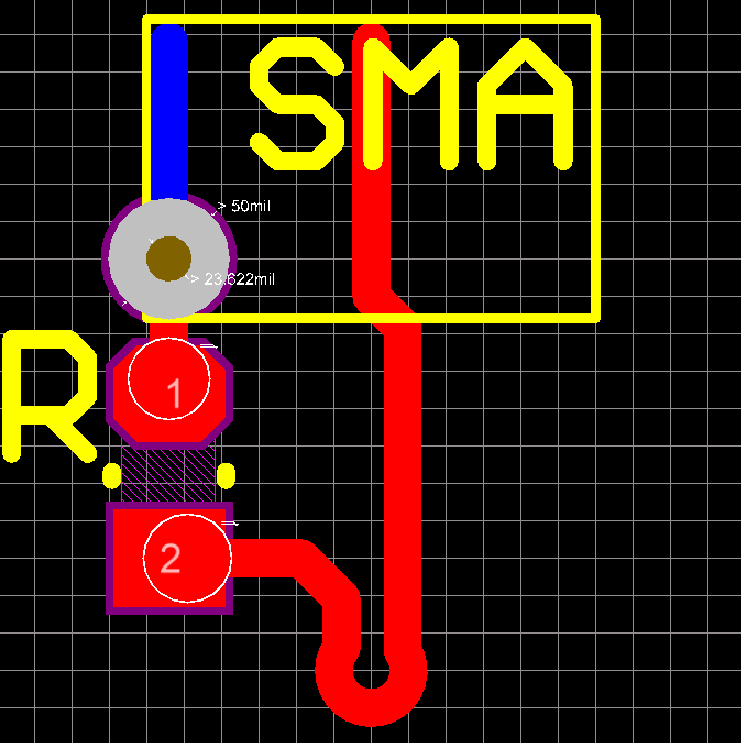
\includegraphics[scale=0.25]{./img/1A_layers}
		\label{fig:1A_layers}}
	\subfloat[][FS05CT]{
		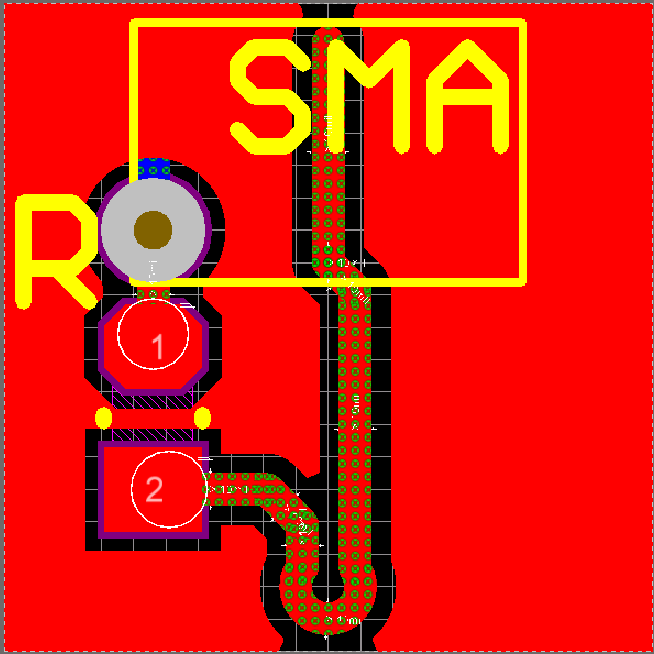
\includegraphics[scale=0.28]{./img/1B_layers}
		\label{fig:1B_layers}}
    \fonte{Elaborado pelo Autor (2019)}
\end{figure}

Na figura~\ref{fig:2A_layers} pode-se visualizar o leiaute desenvolvido para a NFP de face simples com raio de 1mm sem o plano de terra. Na figura~\ref{fig:2B_layers} pode-se visualizar o leiaute desenvolvido para a NFP de face simples com raio de 1mm com o plano de terra.
\begin{figure}[htb!]
	\centering
 	\caption{NFP face simples - 1mm}
	\subfloat[][FS10ST]{
		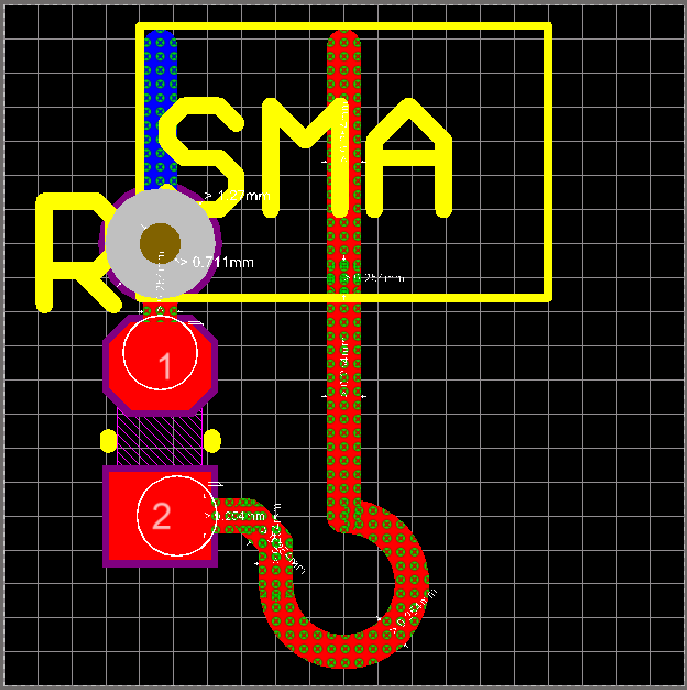
\includegraphics[scale=0.3]{./img/2A_layers}
		\label{fig:2A_layers}}
	\subfloat[][FS10CT]{
		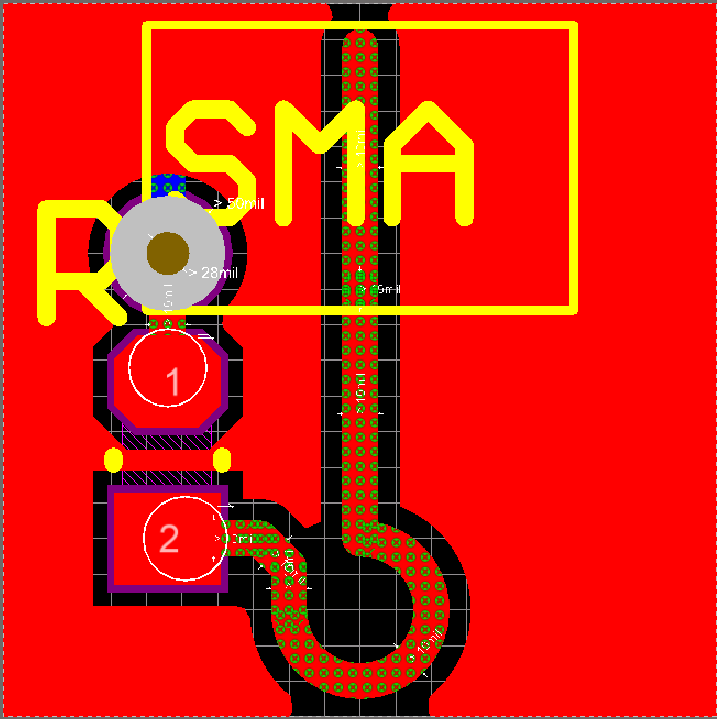
\includegraphics[scale=0.29]{./img/2B_layers}
		\label{fig:2B_layers}}
    \fonte{Elaborado pelo Autor (2019)}
\end{figure}

Na figura~\ref{fig:3A_layers} pode-se visualizar o leiaute desenvolvido para a NFP de face simples com raio de 1.5mm sem o plano de terra. Na figura~\ref{fig:3B_layers} pode-se visualizar o leiaute desenvolvido para a NFP de face simples com raio de 1.5mm com o plano de terra. Como o raios desta NFP ficou 3 vezes maior que as~\ref{fig:1A_layers} e~\ref{fig:1B_layers} notamos que a espira não ficou completa, faltou $\frac{1}{4}$ de volta para realizar a espira completa.
\begin{figure}[htb!]
	\centering
 	\caption{NFP face simples - 1.5mm}
	\subfloat[][FS15ST]{
		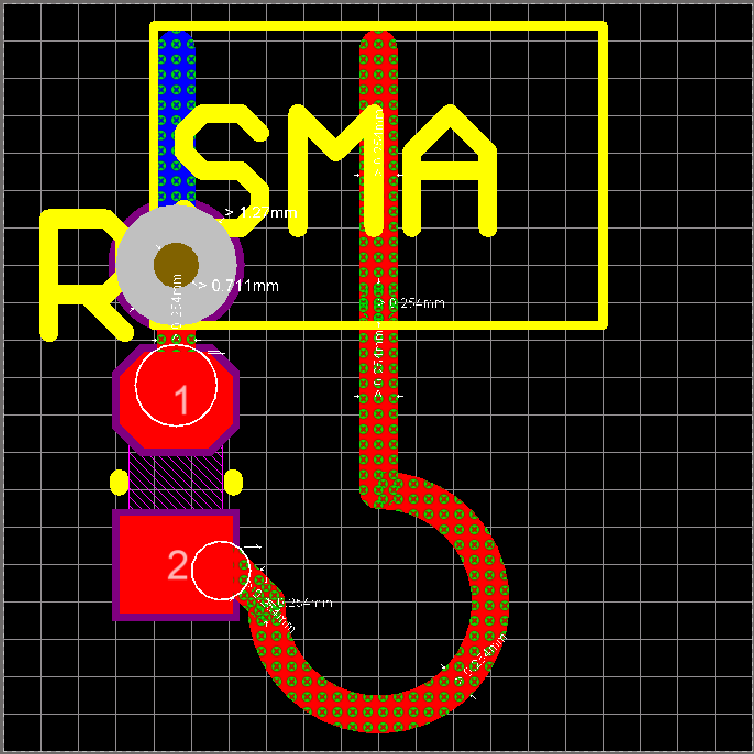
\includegraphics[scale=0.28]{./img/3A_layers}
		\label{fig:3A_layers}}
	\subfloat[][FS15CT]{
		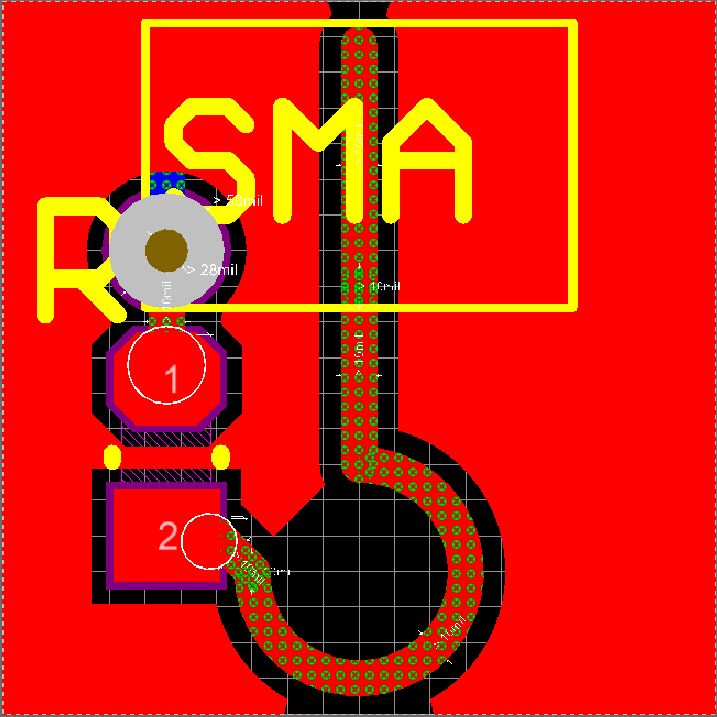
\includegraphics[scale=0.29]{./img/3B_layers}
		\label{fig:3B_layers}}
    \fonte{Elaborado pelo Autor (2019)}
\end{figure}

Na figura~\ref{fig:7A_layers} pode-se visualizar o leiaute desenvolvido para a NFP de face simples com raio de 3mm sem o plano de terra. Na figura~\ref{fig:7B_layers} pode-se visualizar o leiaute desenvolvido para a NFP de face simples com raio de 3mm com o plano de terra. Notamos que nesta NFP a espira ficou quase que completamente fechada.
\begin{figure}[htb!]
	\centering
 	\caption{NFP face simples - 3mm}
	\subfloat[][FS30ST]{
		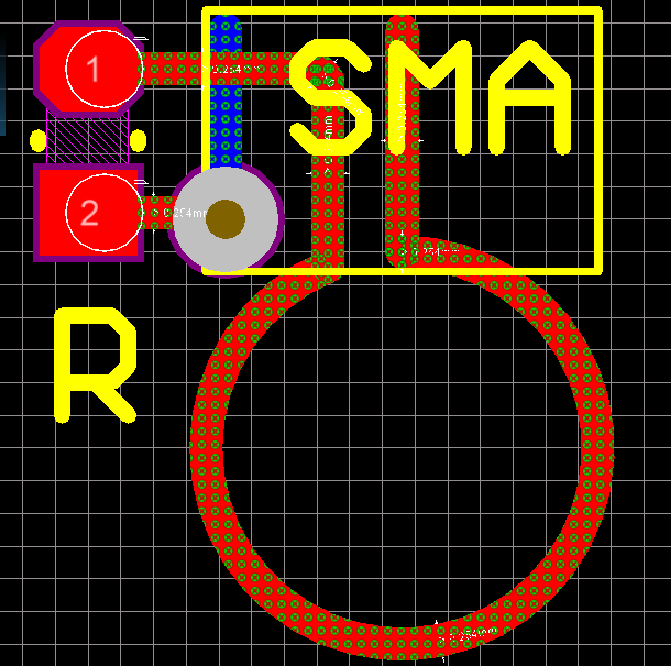
\includegraphics[scale=0.3]{./img/7A_layers}
		\label{fig:7A_layers}}
	\subfloat[][FS30CT]{
		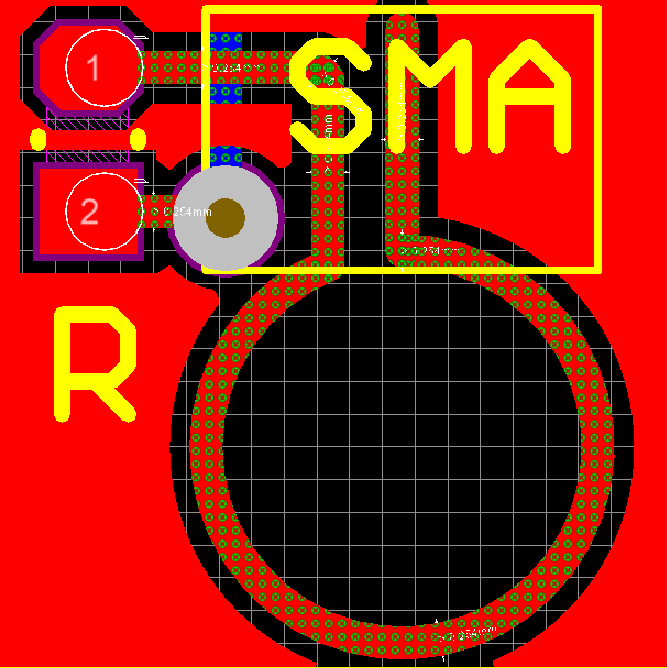
\includegraphics[scale=0.3]{./img/7B_layers}
		\label{fig:7B_layers}}
    \fonte{Elaborado pelo Autor (2019)}
\end{figure}

Na figura~\ref{fig:8A_layers} pode-se visualizar o leiaute desenvolvido para a NFP de face simples com raio de 6mm sem o plano de terra. Na figura~\ref{fig:8B_layers} pode-se visualizar o leiaute desenvolvido para a NFP de face simples com raio de 6mm com o plano de terra. Para esta NFP, devido ao tamanho do raio da espira, foi necessário aumentar as dimensões da PCI, sendo esta a única NFP fora do tamanho adotado como padrão de 10mm por 10mm para as NFPs.
\begin{figure}[htb!]
	\centering
 	\caption{NFP face simples - 6mm}
	\subfloat[][FS60ST]{
		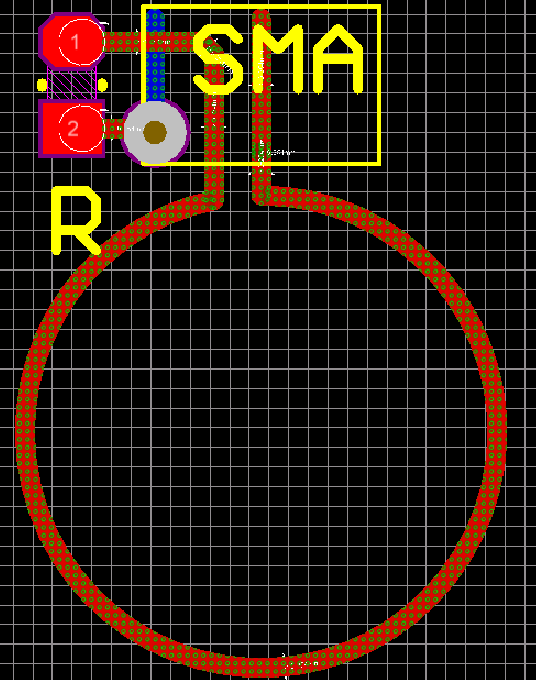
\includegraphics[scale=0.3]{./img/8A_layers}
		\label{fig:8A_layers}}
	\subfloat[][FS60CT]{
		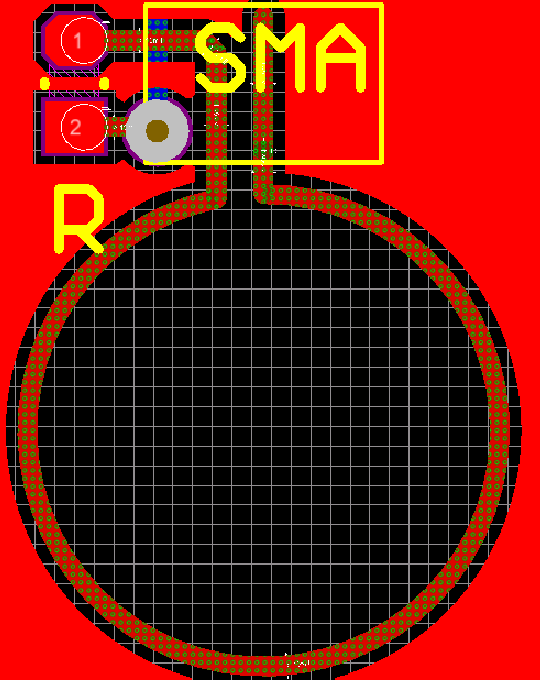
\includegraphics[scale=0.3]{./img/8B_layers}
		\label{fig:8B_layers}}
    \fonte{Elaborado pelo Autor (2019)}
\end{figure}

Desenvolvidas as NFPs de face simples, partiu-se para os leiautes das faces duplas. Na figura~\ref{fig:4A_layers} pode-se visualizar o leiaute desenvolvido para a NFP de face dupla com raio de 0.5mm sem o plano de terra. Na figura~\ref{fig:4B_layers} pode-se visualizar o leiaute desenvolvido para a NFP de face dupla com raio de 0.5mm com o plano de terra. Devido ao fato de necessitar-se de uma via (ligação entre faces) a espira desta NFP assumiu um formato elíptico, preservando-se o menor raio em 0.5mm, no sentido horizontal, porém com uma raio vertical de 2.5mm.
\begin{figure}[htb!]
	\centering
 	\caption{NFP face dupla - 0.5mm}
	\subfloat[][FD05ST]{
		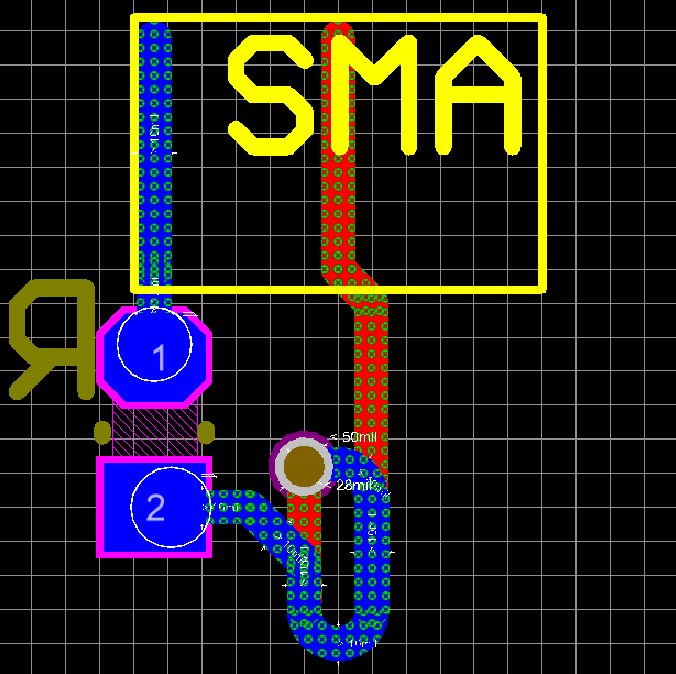
\includegraphics[scale=0.3]{./img/4A_layers}
		\label{fig:4A_layers}}
	\subfloat[][FD05CT]{
		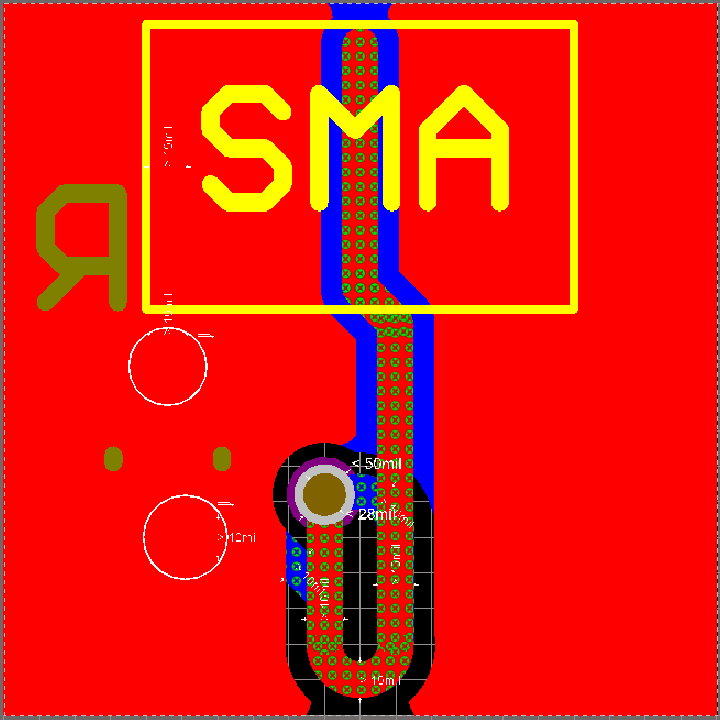
\includegraphics[scale=0.28]{./img/4B_layers}
		\label{fig:4B_layers}}
    \fonte{Elaborado pelo Autor (2019)}
\end{figure}

Na figura~\ref{fig:5A_layers} pode-se visualizar o leiaute desenvolvido para a NFP de face dupla com raio de 1mm sem o plano de terra. Na figura~\ref{fig:5B_layers} pode-se visualizar o leiaute desenvolvido para a NFP de face dupla com raio de 1mm com o plano de terra. 
\begin{figure}[htb!]
	\centering
 	\caption{NFP face dupla - 1mm}
	\subfloat[][FD10ST]{
		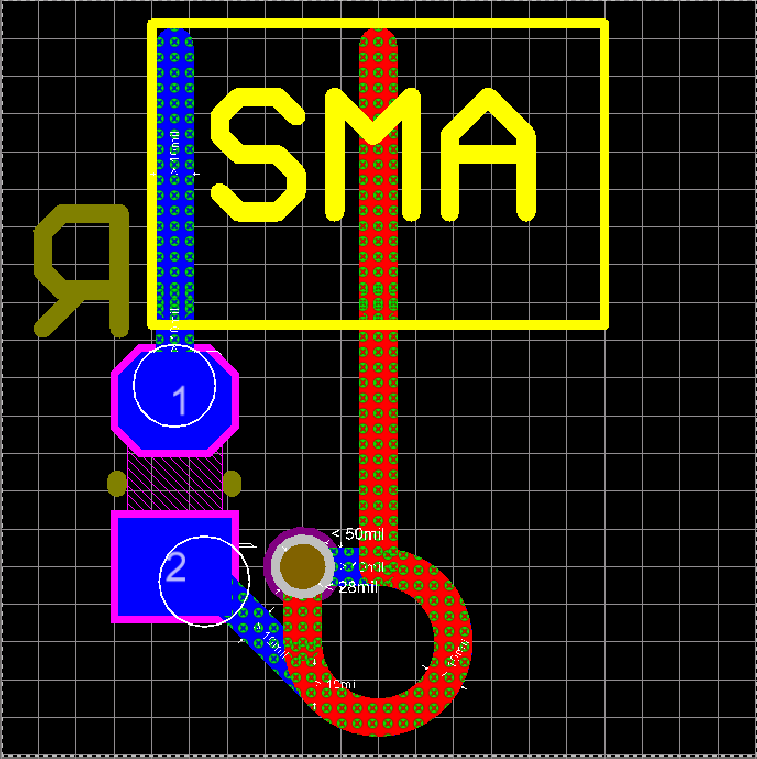
\includegraphics[scale=0.28]{./img/5A_layers}
		\label{fig:5A_layers}}
	\subfloat[][FD10CT]{
		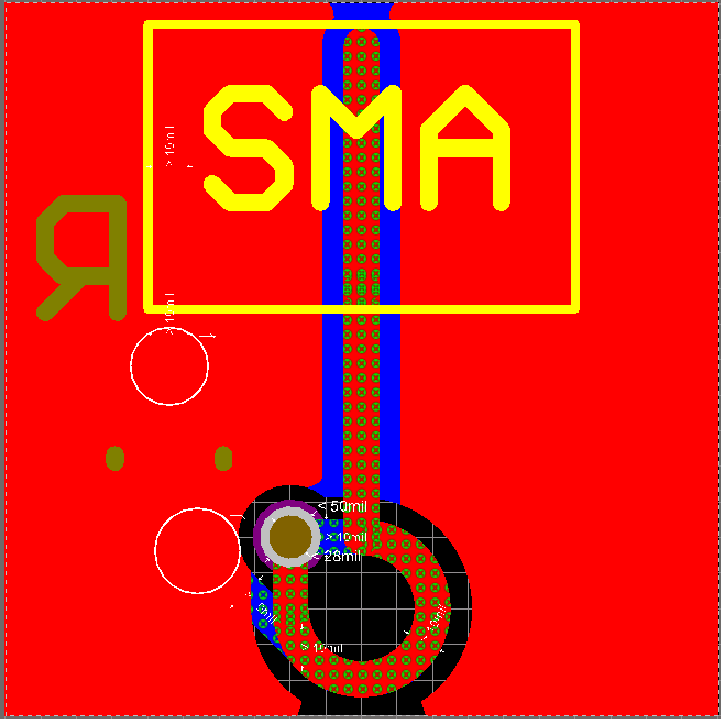
\includegraphics[scale=0.29]{./img/5B_layers}
		\label{fig:5B_layers}}
    \fonte{Elaborado pelo Autor (2019)}
\end{figure}

Na figura~\ref{fig:6A_layers} pode-se visualizar o leiaute desenvolvido para a NFP de face dupla com raio de 1.5mm sem o plano de terra. Na figura~\ref{fig:6B_layers} pode-se visualizar o leiaute desenvolvido para a NFP de face dupla com raio de 1.5mm com o plano de terra. Diferentemente do grupo de face simples, nota-se aqui que as NFPs de face duplas, em pelo menos 1 (uma) espira tem-se a volta completa. 
\begin{figure}[htb!]
	\centering
 	\caption{NFP face dupla - 1.5mm}
	\subfloat[][FD15ST]{
		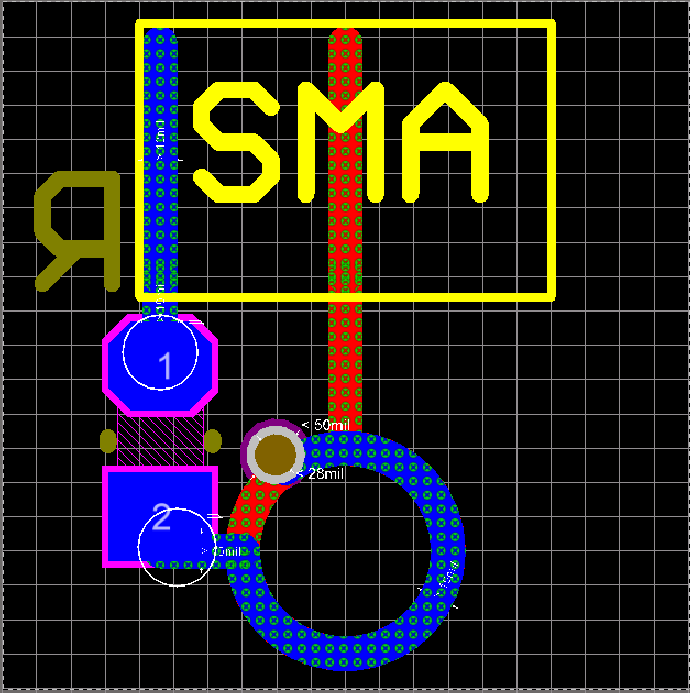
\includegraphics[scale=0.3]{./img/6A_layers}
		\label{fig:6A_layers}}
	\subfloat[][FD15CT]{
		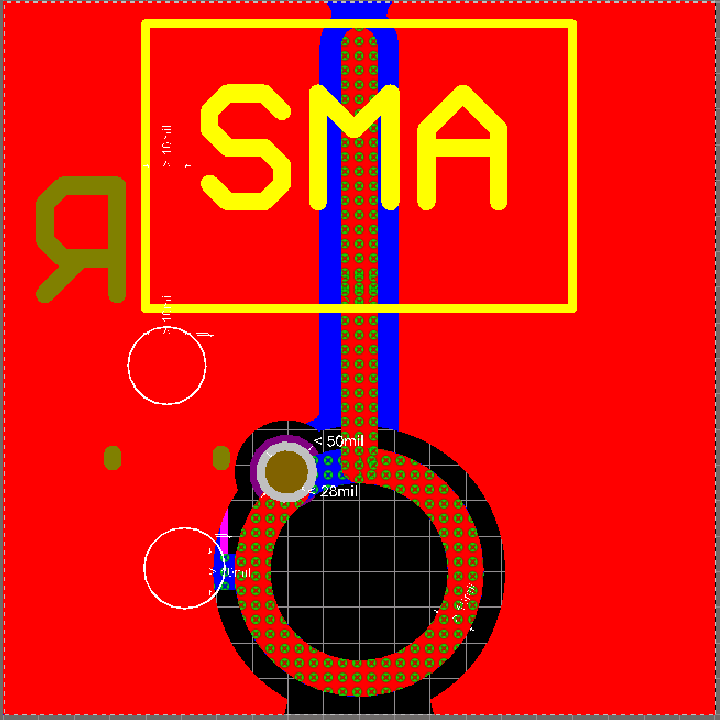
\includegraphics[scale=0.29]{./img/6B_layers}
		\label{fig:6B_layers}}
    \fonte{Elaborado pelo Autor (2019)}
\end{figure}

Na figura~\ref{fig:9A_layers} pode-se visualizar o leiaute desenvolvido para a NFP de face dupla com raio de 3mm sem o plano de terra. Na figura~\ref{fig:9B_layers} pode-se visualizar o leiaute desenvolvido para a NFP de face dupla com raio de 3mm com o plano de terra. 
\begin{figure}[htb!]
	\centering
 	\caption{NFP face dupla - 3mm}
	\subfloat[][FD30ST]{
		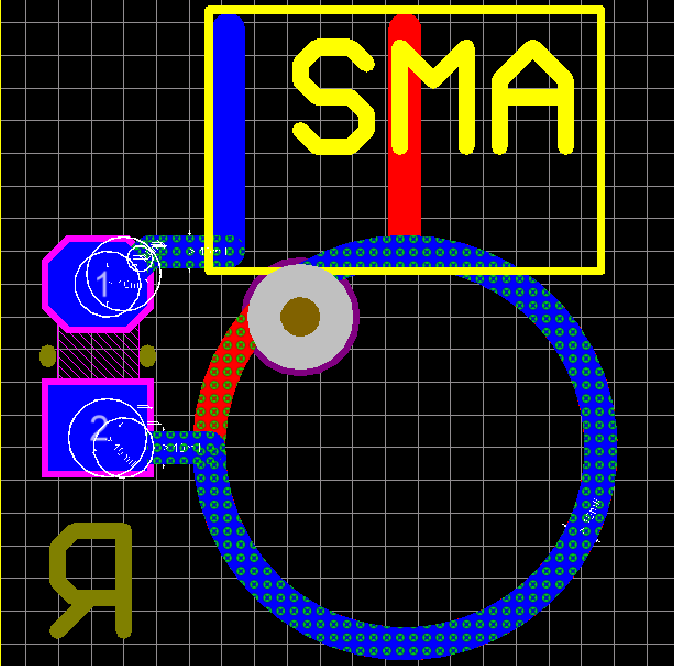
\includegraphics[scale=0.3]{./img/9A_layers}
		\label{fig:9A_layers}}
	\subfloat[][FD30CT]{
		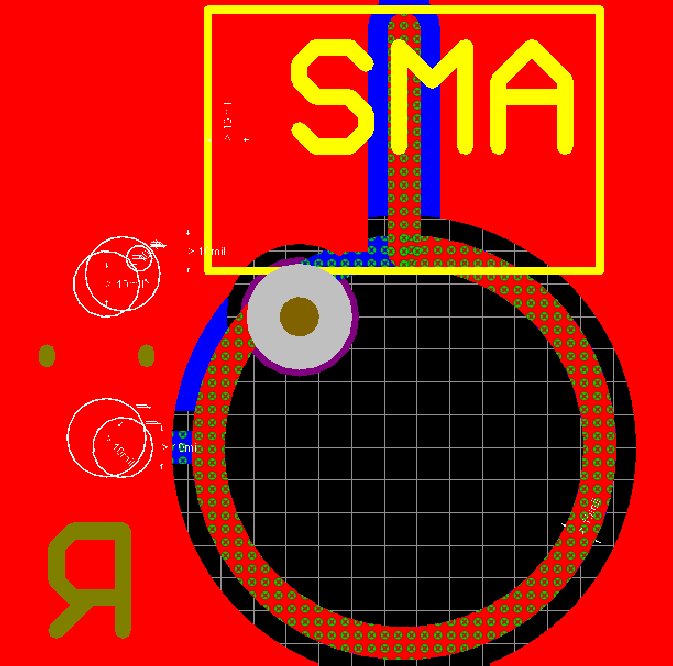
\includegraphics[scale=0.3]{./img/9B_layers}
		\label{fig:9B_layers}}
    \fonte{Elaborado pelo Autor (2019)}
\end{figure}

E por fim, na figura~\ref{fig:10A_layers} pode-se visualizar o leiaute desenvolvido para a NFP de face dupla com raio de 6mm sem o plano de terra. Na figura~\ref{fig:10B_layers} pode-se visualizar o leiaute desenvolvido para a NFP de face dupla com raio de 6mm com o plano de terra. 
\begin{figure}[htb!]
	\centering
 	\caption{NFP face dupla - 6mm}
	\subfloat[][FD60ST]{
		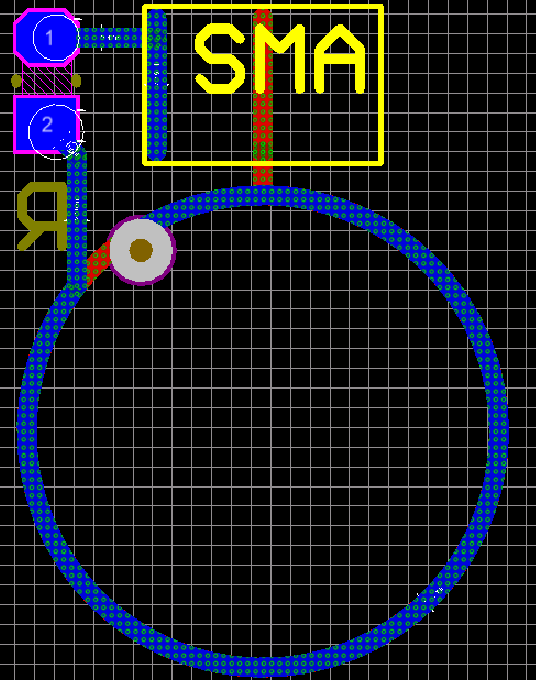
\includegraphics[scale=0.3]{./img/10A_layers}
		\label{fig:10A_layers}}
	\subfloat[][FD60CT]{
		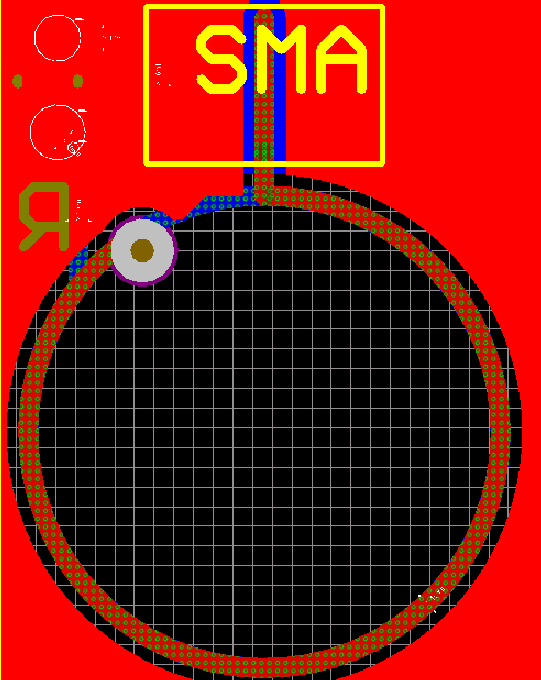
\includegraphics[scale=0.3]{./img/10B_layers}
		\label{fig:10B_layers}}
    \fonte{Elaborado pelo Autor (2019)}
\end{figure}

As maiores dificuldades nos projetos das NFPs, de forma geral, foi a alocação da carga resistiva de $50\Omega$ (Casamento de impedância) e alocar a via (ligação interfaces), esses pequenos empecilhos acarretaram na imperfeição do formato circular, fechado, das espiras, para as NFPs de raios menores que 1.5mm.

% Na figura~\ref{fig:Single_PCI_project} visualiza-se o conjunto de NFPs de face simples preparadas para a fabricação bem como na figura~\ref{fig:Double_PCI_project} visualiza-se o conjunto de NFPs de face dupla também preparadas para a fabricação
% \begin{figure}[htb!]
% 	\centering
%  	\caption{Projeto das NFPs - Fabricação}
% 	\subfloat[][NFPs de Face Simples]{
% 		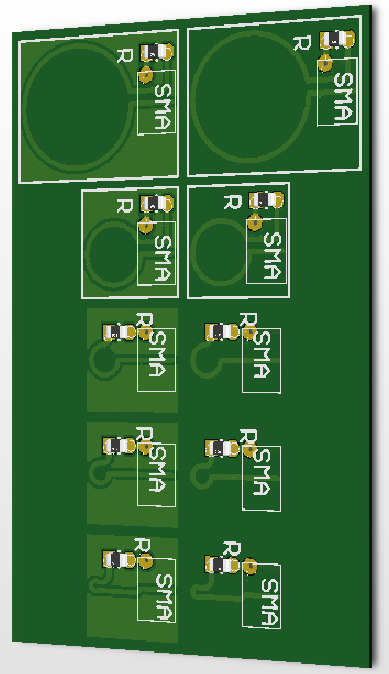
\includegraphics[scale=0.5]{./img/Single_PCI_project}
% 		\label{fig:Single_PCI_project}}
% 	\subfloat[][NFPs de Face Dupla]{
% 		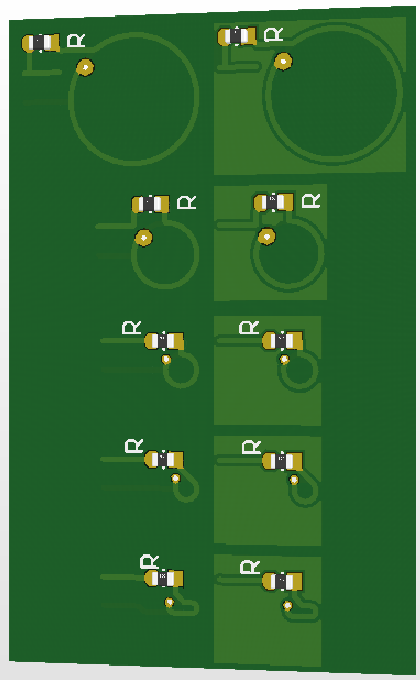
\includegraphics[scale=0.5]{./img/Double_PCI_project}
% 		\label{fig:Double_PCI_project}}
%     \fonte{Elaborado pelo Autor (2019)}
% \end{figure}

\begin{figure}[htb!]
	\centering
 	\caption{NFPs Elaboradas}
	\subfloat[][NFPs de Face Simples]{
		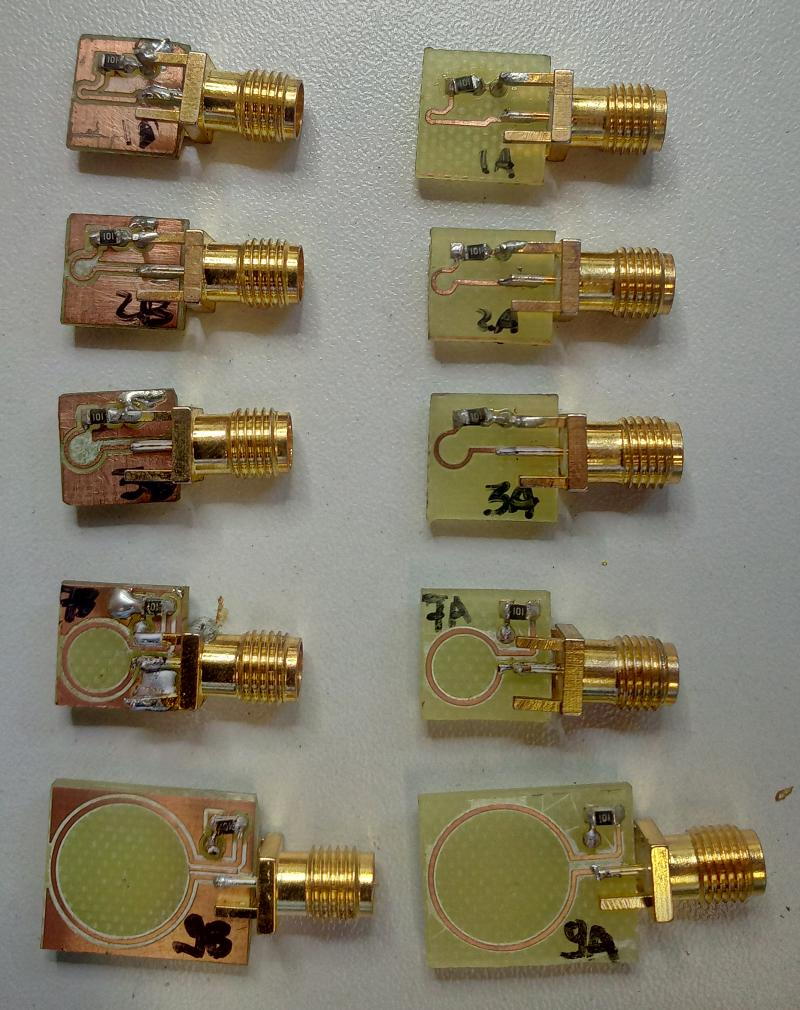
\includegraphics[scale=0.4]{./img/singlefaceNFPS}
		\label{fig:singlefaceNFPS}}
	\subfloat[][NFPs de Face Dupla]{
		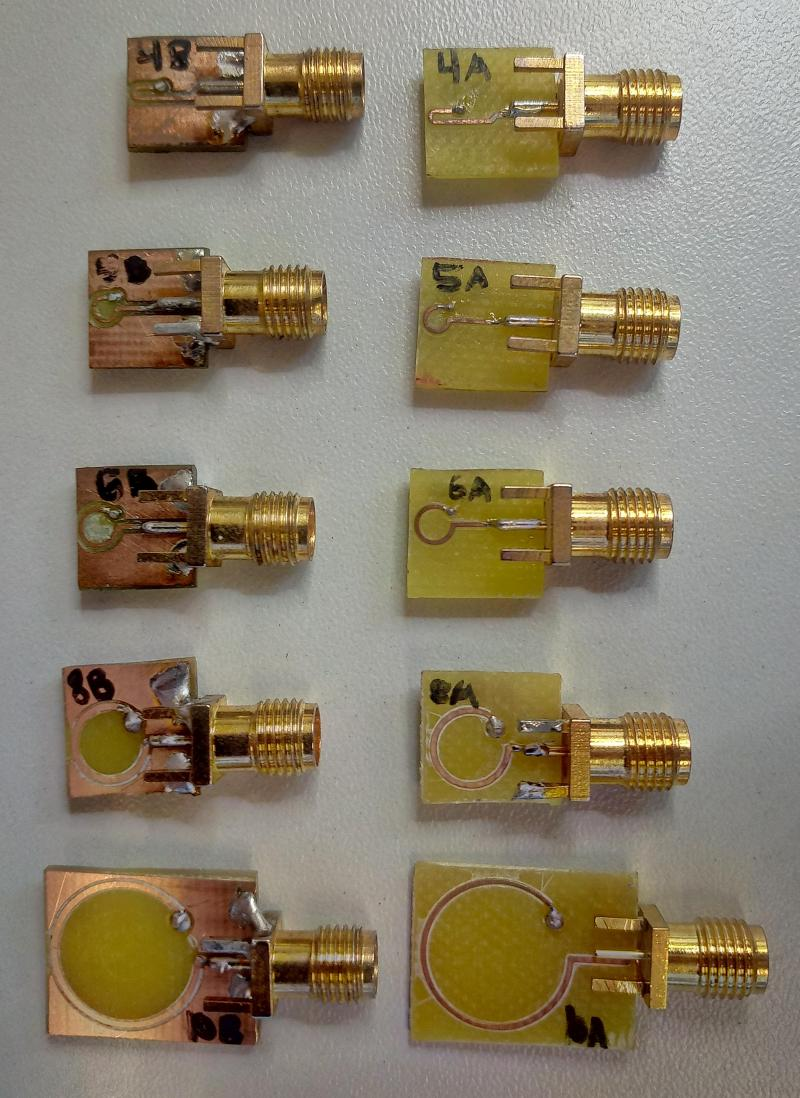
\includegraphics[scale=0.37]{./img/doublefaceNFPS}
		\label{fig:doublefaceNFPS}}
    \fonte{Elaborado pelo Autor (2019)}
\end{figure}

Após a fabricação e montagens o aspecto final das NFPs pode ser visto nas figuras~\ref{fig:singlefaceNFPS} e ~\ref{fig:doublefaceNFPS} de face simples e dupla respectivamente.

\section{Esquemas de medidas e procedimentos}
Para a realização dos experimentos seria necessário, idealmente, ter um sistema de posicionamento XY, porém este sistema de posicionamento será tratado em outro estudo desenvolvido no LabCEM do departamento de eletrônica do IFSC. Assim para realizar as experimentações desenvolveu-se um suporte fixo em madeira (para não interferir nas radiações eletromagnéticas) em que o posicionamento da NFP se deu de forma manual.

\begin{figure}[htb!]
	\centering
 	\caption{Suporte Fixo para posicionamento das NFPs}
	\subfloat[][Visão Superior]{
		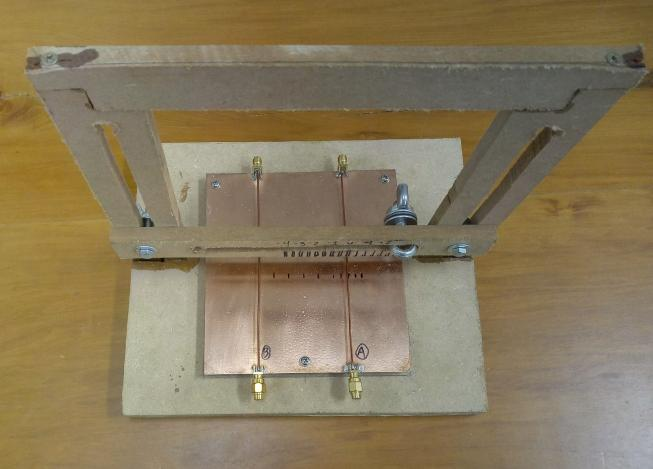
\includegraphics[scale=0.5]{./img/suporteTOP}
		\label{fig:suporteTOP}}
	\subfloat[][Visão Frontal]{
		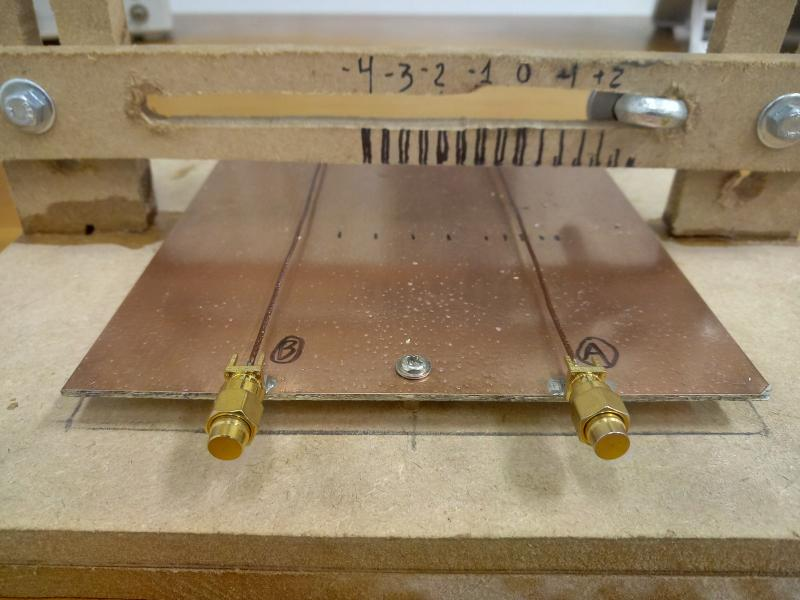
\includegraphics[scale=0.39]{./img/suporteFRONT}
		\label{fig:suporteFRONT}}
    \fonte{Elaborado pelo Autor (2019)}
\end{figure}

Na figura~\ref{fig:suporteTOP} podemos visualizar a vista superior do suporte, onde vemos que o mesmo foi projetado para haver movimentos tanto na direção vertical, onde definiu-se com eixo z, quanto na direção horizontal, definido com eixo y. Vemos também que na base do suporte, em plano fixo, foi alocado o dispositivo sob teste (DUT), mais a frente será detalhado o modelo de DUT utilizado.

Na figura~\ref{fig:suporteFRONT} pode-se visualizar a vista frontal do suporte, onde vemos as marcações para o posicionamento lateral de afastamento, na direção horizontal. Destaca-se aqui que foi adotado o sentido da esquerda para a direita como posições positivas, tomando como referência zero (0mm) o ponto acima do DUT(A), dessa forma, posições mais a direita são valores positivos e posições mais a esquerda são valores negativos.

\subsection{Modelo para o dispositivo sob teste - DUT}
Para implementar um dispositivo sob teste, ou DUT, tomou-se por referência o adotado por~\citeonline[p.~39]{sivaraman2017} porém, para realizar o experimento de caracterização de resolução espacial por DUT duplo, acrescentou-se dois DUTs sob o mesmo plano de terra. Na figura~\ref{fig:esquema3_fundo} visualiza-se os DUTs, que são compostos de dois fios de cobre esmaltados dispostos acima de uma plano de terra, numa distância média de $h = 3mm$, tendo os fios um raio $r = 0,512mm$ ou $18AWG$ separados entre si por uma distância de $D = 60mm$. Em cada fio, numa de suas extremidades esta um conector SMA \textit{SubMiniature version A} - Conector Coaxial de RF de $50\Omega$) e na outra uma carga resistiva de $50\Omega$ ligando o fio ao plano de terra.

\begin{figure}[htb!]
	\centering 
	\caption{Modelo de DUT}
	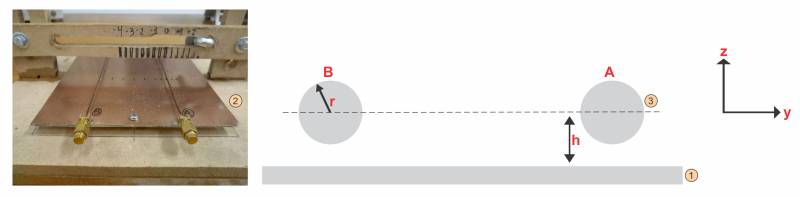
\includegraphics[scale=2.4]{./img/esquema3_fundo}
	\fonte{Elaborado pelo Autor (2019)}
	%\legend{\hspace{-218pt}Fonte:~\citeonline[p.~8]{paul2006}}
	\label{fig:esquema3_fundo}
\end{figure}

Na figura~\ref{fig:esquema3_fundo} vemos marcado em (1) o plano de terra em (2) o DUT real desenvolvido, em (3) o modelo para os fios de cobre esmaltados e ainda vemos uma referência indicativa das direções positivas e eixos adotados nas medições que serão vistas a frente.

%Colocar modelo do circuito elétrico equivalente

\subsection{Equipamentos do laboratório}
Além do suporte e do DUT desenvolvidos, foi necessário a utilização de alguns equipamentos do LabCEM do departamento de eletrônica do IFSC. na figura~\ref{fig:esl} vemos o analisador de espectro da Rohde \& Schwarz modelo ESL3 que foi utilizado para a caracterização da resposta em frequência de 5MHz até 3GHz das NFPs, além da NFP comercial, cujo será realizado uma comparação de performance. Este analisador tem entre as principais características (de interesse para este trabalho) uma faixa de operação de frequência de 9kHz até 3GHz e um gerador de rastreamento com faixa de operação de 1MHz até 3GHz.

\begin{figure}[htb!]
	\centering
 	\caption{Analisadores de Espectro - LabCEM}
	\subfloat[][Analisador ESL]{
		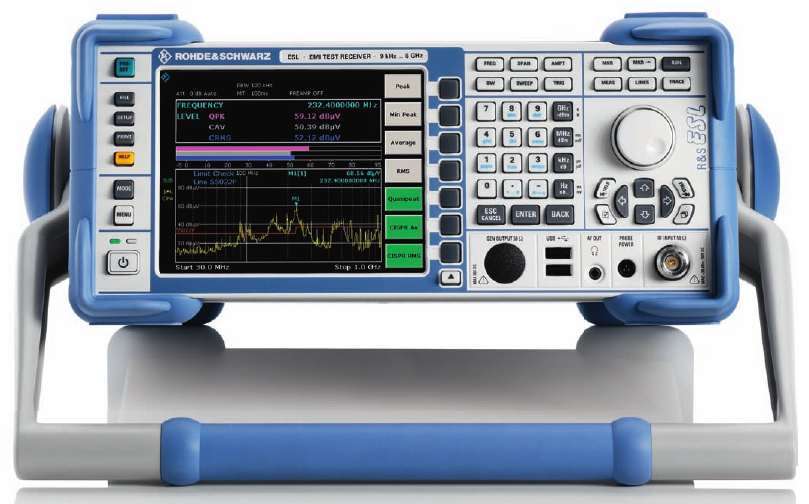
\includegraphics[scale=0.4]{./img/esl}
		\label{fig:esl}}
	\subfloat[][Analisador HMS-X]{
		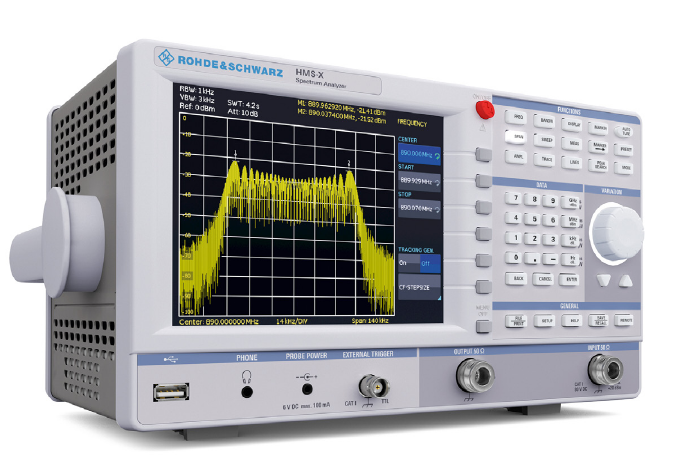
\includegraphics[scale=0.4]{./img/HMS-X}
		\label{fig:HMS-X}}
    \fonte{Elaborado pelo Autor (2019)}
\end{figure}

Outro analisador utilizado é demonstrado na figura~\ref{fig:HMS-X}, também da Rohde \& Schwarz no modelo HMS-X, sendo este utilizado na caracterização em baixas frequências, intensidade por distância e resolução espacial das NFPs com DUT duplo. Este analisador tem entre as principais características (de interesse para este trabalho) uma faixa de operação de frequência de 0Hz até 1.6GHz.

\section{Caracterização da Resposta em Frequência}
O procedimento adotado na caracterização da resposta em frequência consistiu em posicionar cada NFP exatamente sob o DUT(A) (em 0mm, no eixo y) em uma distância de aproximadamente 1mm (eixo z) em relação ao DUT(A), configurou-se o analisador ESL3 para operar no modo gerador de rastreamento (\textit{Tracking generator}), selecionado a frequência inicial em 5MHz e a final em 3GHz, com isso obteve-se a curva de resposta em frequência para cada NFP. Além deste procedimento, também foi realizado a exportação dos dados capturados pelo analisador, afim de realizador um melhor tratamento dos dados via MatLab.

Todas as medidas foram coletadas utilizando a seguinte configuração padrão, RBW = 10kHz, VBW = 100kHz, Ref = 107 $dB \mu V$, tempo de varredura (SWT) = 100ms e Atenuação (Att) = 10dB. Sendo que RBW significa \textit{Resolution Bandwidth} que determina quão próximos dois sinais no domínio da frequência podem ser visualizados. VBW é o \textit{Video Bandwidth} que define a capacidade de discernirem-se dois níveis de potências distintos, uma vez que o sinal digitalizado armazenado pode ser a média de vários pontos próximos.

% Incluir o preset adotado --> RBW; RBW, Ref, sweet, Attenuation, etc...

% Resolução Largura de Banda é uma medida qualitativa da separação mínima necessária entre dois componentes de frequência para poder separá-los visualmente e, para o VSA, é definida como a Largura de Banda de Ruído Equivalente do filtro, que é determinada pelo tipo de janela selecionado e o comprimento da janela.
% 
% Largura de banda de resolução (ResBW ou RBW) afeta o seguinte:
% 
% A resolução de frequência para traços de espectro
% Quão rápido o VSA faz uma medição
% Parâmetro ResBW: especifica o RBW de medição. O VSA ajustará o RBW ao valor mais próximo que satisfaça a configuração de medição atual.
% 
% Como a largura de banda de resolução está diretamente relacionada ao tempo de medição, a seleção manual de uma largura de banda de resolução mais restrita pode atrasar a medição mais do que o necessário. Por outro lado, a seleção de uma largura de banda de resolução muito ampla pode não fornecer a resolução adequada e obscurecer os componentes espectrais que estão próximos uns dos outros.

% 
% O tempo de varredura da tela em um equipamento de medição é afetado por ambas larguras de faixa. Se o VBW for menor que o RBW, o tempo de varredura t_{sweep} é dado por [2]:
% 
% t_{sweep}=\frac{k(f_{2}-f_{1})}{RBW \times VBW}
% 
% onde k é uma constante que depende da construção do equipamento e f2-f1 é a faixa de frequência mostrada na tela.

%Outro procedimento adotado foi a caracterização da resposta em frequência do DUT(A), no intuito de utilizar os dados para anular, via MatLab, o efeito do DUT(A) na respostas das NFPs. 
Também procedeu-se com a caracterização da resposta em frequência de uma NFP comercial, com a intenção de realizar uma comparação com as NFPs produzidas.

\begin{figure}[htb!]
	\centering 
	\caption{Esquema de ligações para medidas - Resposta em Frequência}
	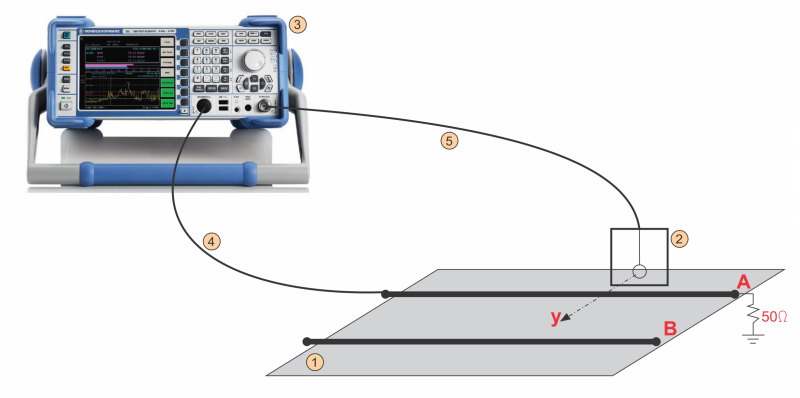
\includegraphics[scale=2.4]{./img/esquema2_fundo}
	\fonte{Elaborado pelo Autor (2019)}
	%\legend{\hspace{-218pt}Fonte:~\citeonline[p.~8]{paul2006}}
	\label{fig:esquema2_fundo}
\end{figure}

Na figura~\ref{fig:esquema2_fundo} pode-se visualizar o esquema de ligação utilizado neste procedimento, onde na marcação (1) temos o plano de terra do DUT(A) e (B), em (2) temos a NFP posicionada, em (3) temos o analisador ESL3, e por fim (4) e (5) vemos os cabos de ligação de saída e entrada respectivamente.

%\subsection{Caracterização da Resposta em Baixas Frequências}
\section{Caracterização da Intensidade por distância}
No intuito de investigar a resolução espacial das NFPs, procedeu-se com a coleta de medidas de intensidade de leitura da NFP pela distância lateral em relação ao DUT, em ~\citeonline[p.~54]{sivaraman2017} adotou-se este procedimento. Como no IFSC não há geradores de funções com capacidade de gerar sinusoides em frequências maiores de que 25MHz, definiu-se por trabalhar na faixa de 5MHz e 25MHz, dentro das possibilidades que os equipamentos disponíveis poderiam entregar.

Para efetuar esta caracterização, na faixa de operação de 5MHz até 25MHz, utilizou-se dois equipamentos, um gerador de função configurado para gerar um sinal sinusoidal de 2Vpp com possibilidade de alterar a frequência na faixa desejada e o analisador de espectro HMS-X capturando a intensidade do sinal obtido na NFP. Foi-se alterando o posicionamento da NFP de 10mm em 10mm em cada direção (positiva e negativa) do eixo y, sendo que em cada posição anotou-se os valores de intensidade $dB\mu V$ para as frequências de 5MHz, 10MHz, 15MHz, 20MHz e 25MHz.

\begin{figure}[htb!]
	\centering 
	\caption{Esquema de Ligações para Medidas - Resposta em Baixas Frequência}
	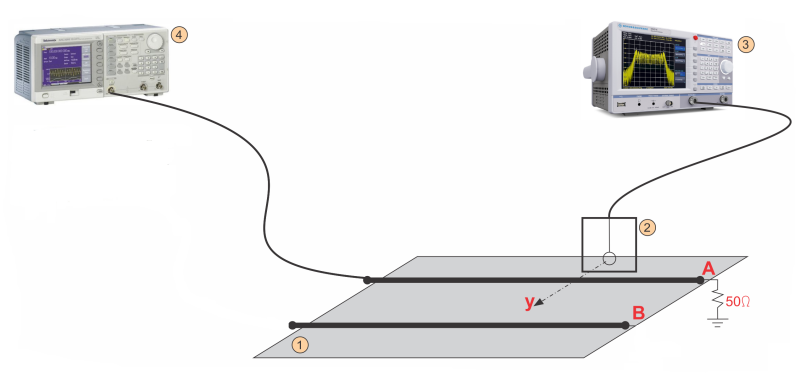
\includegraphics[scale=2.4]{./img/esquema4_fundo}
	\fonte{Elaborado pelo Autor (2019)}
	%\legend{\hspace{-218pt}Fonte:~\citeonline[p.~8]{paul2006}}
	\label{fig:esquema4_fundo}
\end{figure}

Na figura~\ref{fig:esquema4_fundo} pode-se visualizar o esquema de ligação utilizado neste procedimento, onde na marcação (1) temos o plano de terra do DUT(A) e (B), em (2) temos a NFP posicionada, em (3) temos o analisador HMS-X, e por fim em (4) o gerador de função que estará impondo uma senoide de 2Vpp.
%Segunda Leva de Resultados, outra perspectiva da primeira

%Nesta etapa de caracterizações, o procedimento adotado consistiu na utilização do mesmo esquema de montagem visualizado na figura~\ref{fig:esquema4_fundo}, porém foi-se alterando o posicionamento da NFP de 10mm em 10mm em cada direção (positiva e negativa) do eixo y, sendo que em cada posição anotou-se os valores de intensidade $dB\mu V$ para as frequências de 5MHz, 10MHz, 15MHz, 20MHz e 25MHz. Destaca-se que os valores obtidos nessa etapa são os mesmos utilizados na visualização da resposta em frequência, onde ambas as medidas são iguais, apenas utilizou-se perspectivas de análise ou visualização diferentes.

%Primeira Leva de Resultados.

\section{Caracterização da Resolução Espacial - DUT Duplo}
Neste caso, foi necessário a inclusão de um segundo gerador de função, dessa forma teve-se dois DUTs operando simultaneamente, em frequências diferentes, sob o mesmo plano de terra, dessa forma inferiu-se experimentalmente o comportamento de cada NFP em relação a resolução espacial, operando com duas frequências em conjunto. Similarmente as caracterizações anteriores, foi-se alterando o posicionamento da NFP de 10mm em 10mm, porém somente no sentido à esquerda (negativo em y), sendo que em cada posição anotou-se os valores de intensidade $dB\mu V$ para as frequências dos sinais inseridos nos DUTs, sendo que no DUT(A) inseriu-se um sinal sinusoidal de 2Vpp em 20MHz, e no DUT(B) um sinal sinusoidal de 2Vpp em 25MHz

\begin{figure}[htb!]
	\centering 
	\caption{Esquema de Ligações para Medidas - DUT Duplo}
	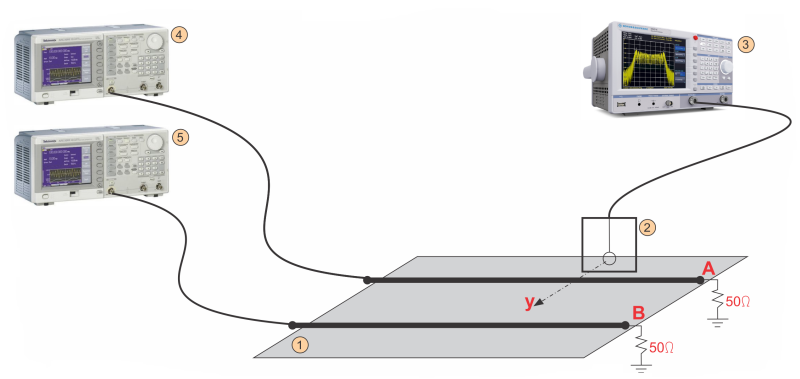
\includegraphics[scale=2.4]{./img/esquema1_fundo}
	\fonte{Elaborado pelo Autor (2019)}
	%\legend{\hspace{-218pt}Fonte:~\citeonline[p.~8]{paul2006}}
	\label{fig:esquema1_fundo}
\end{figure}

Na figura~\ref{fig:esquema1_fundo} pode-se visualizar o esquema de ligação utilizado neste procedimento, onde na marcação (1) temos o plano de terra do DUT(A) e (B), em (2) temos a NFP posicionada, em (3) temos o analisador HMS-X, em (4) o gerador de função que estará impondo uma senoide de 2Vpp de 20MHz no DUT(A) e por fim em (5) o gerador de função que estará impondo uma senoide de 2Vpp de 25MHz no DUT(B).

% \section{Caracterização dos paramentros essencias}
% 
% \subsection{Fator de Antena}
% 
% \subsubsection*{Leiaoutes de face simples}
% 
% \subsubsection*{Leiaoutes de face supla}
% 
% 
% \subsection{Sensitividade}
% 
% \subsubsection*{Leiaoutes de face simples}
% 
% \subsubsection*{Leiaoutes de face supla}
% 
% 
% \subsection{Seletividade}
% 
% \subsubsection*{Leiaoutes de face simples}
% 
% \subsubsection*{Leiaoutes de face supla}
% 
% 
% \subsection{Resolução Especial}
% 
% \subsubsection*{Leiaoutes de face simples}
% 
% \subsubsection*{Leiaoutes de face supla}
% 
% 
% \subsection{Largura de Banda}
% 
% \subsubsection*{Leiaoutes de face simples}
% 
% \subsubsection*{Leiaoutes de face supla}

